\chapter{Versuchsdurchführung}
    \section{Aufnahme der Eingangskennlinie}
        Für die Aufnahme der Eingangskennlinie  eines Transistors wird folgende Schaltung benötigt \fref{fig:21}. 
        Dabei wurde die Schaltung aus dem Versuchsaufbau etwas vereinfacht.

        \begin{figure}[!ht]
            \centering
            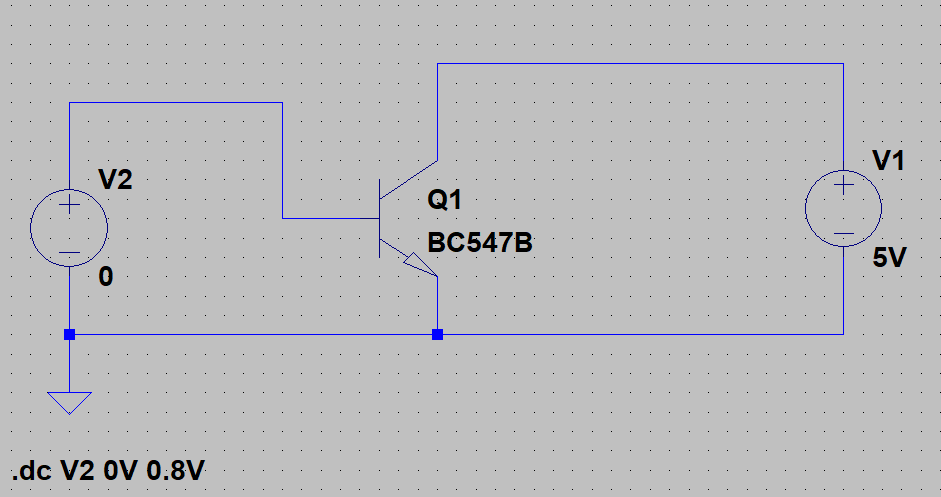
\includegraphics[width=0.5\linewidth]{Bilder/21aufbau.PNG}
            \caption{Schaltung zur Aufnahme der Eingangskennlinie}
            ~\label{fig:21}
        \end{figure}

        Für V1(\(U_{CE}\)) werden 5V verwendet und V2(\(U_{BE}\)) wird im Intervall zwischen 0V und 0,8V verwendet. Bei der Messung des Basisstrom \(I_B\) kamen folgende Werte heraus, welche in einem Graph dargestellt sind.

        \begin{figure}[!ht]
            \centering
                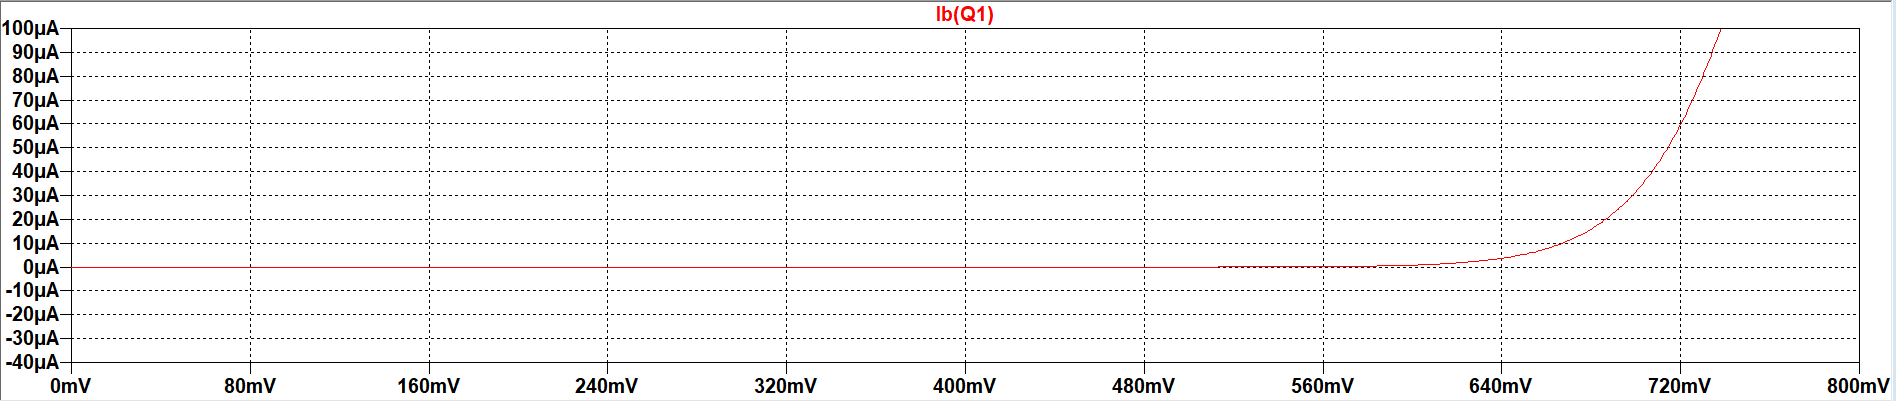
\includegraphics[width=\linewidth]{Bilder/21graph.PNG}
            \caption{Messwerte des Eingangssignals eines NPN-Transistors (Typ BC547B)}
        \end{figure}

        Der Basisstrom eines NPN-Transistors liegt bei 0A bis bis er circa bei einer Spannung von 640mV stark ansteigt.

        \newpage
    \section{Bestimmung des differentiellen Eingangswiderstands}
        Zur Bestimmung des differentiellen Eingangswiderstandes (\(r_{BE}\)) wird die Schaltung aus 2.1 leicht verändert. Die Spannungsquelle V2 wird durch eine Stromquelle I1 ersetzt. Die Spannungsquelle V1 bleibt bei 5V und I1 (\(I_B\)) wird im Intervall von \(10nA\) bis \(100\mu A\) eingesetzt. 

        \begin{figure}[!ht]
        \centering
        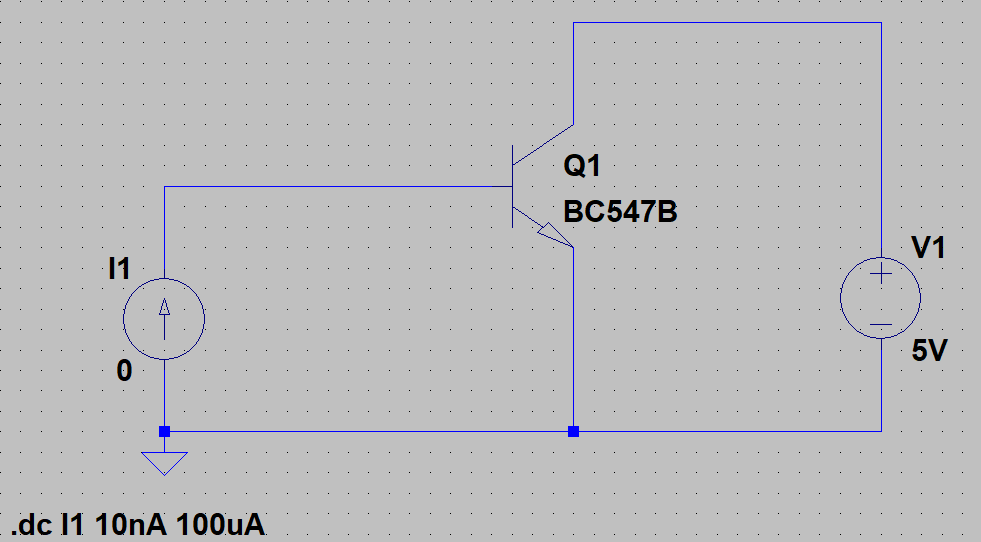
\includegraphics[width=0.5\linewidth]{Bilder/22aufbau.PNG}
        \caption{Schaltung zur Aufnahme des Eingangswiderstandes}
        \label{fig:22}
        \end{figure}

        Durch das Simulieren mit LT-Spice erhalten wir folgenden Graphen für den Eingangswiderstand. Die Werte sind doppellogarithmisch aufgetragen.

        \begin{figure}[!ht]
            \centering
            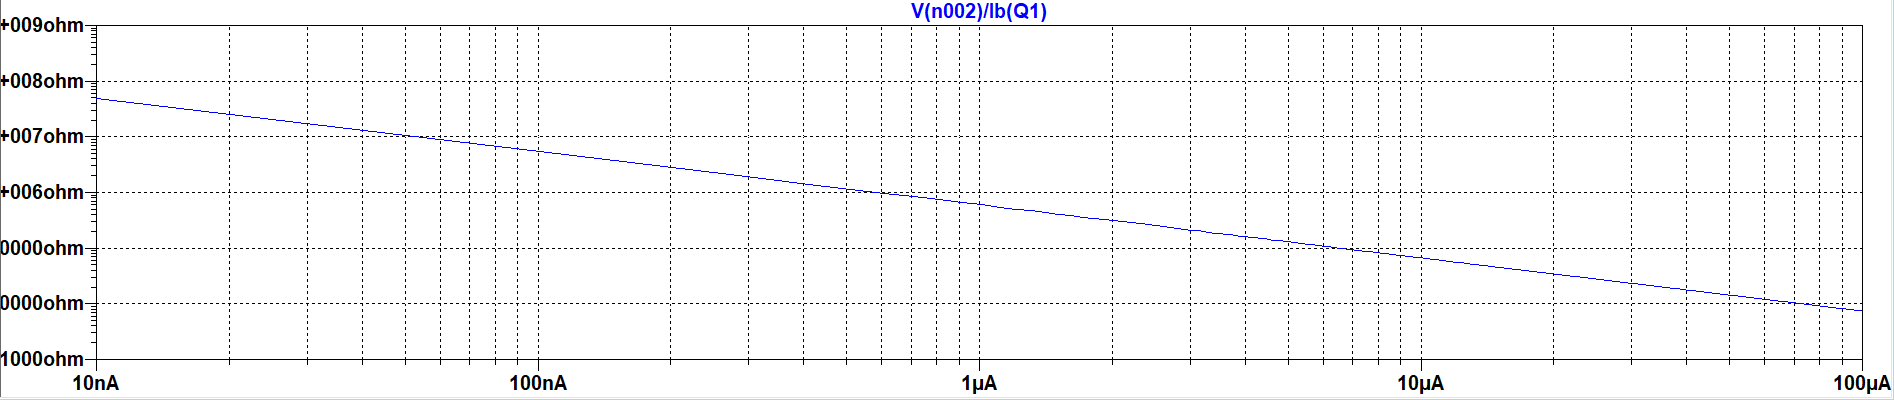
\includegraphics[width=\linewidth]{Bilder/22graph.PNG}
            \caption{Messwerte für \(r_{BE}=f(I_B)\)}
        \end{figure}

        Im Graphen ist zu erkennen, das der Eingangswiderstand mit steigender Stromstärke sinkt.

        \newpage
    \section{Aufnahme der Stromsteuerkennlinie}
        Um die Stromsteuerkennlinie \(I_C=f(I_B)\) zu ermitteln wird die selbe Schaltung verwendet \fref{fig:22}. Die Spannungsquelle V1 wird wieder mit 5V versorgt. \(I_B\) wird dabei im Intervall von \(1\mu A\) bis \(1mA\) in der Simulation mit LT-Spice verändert. 

        \begin{figure}[!ht]
            \centering
            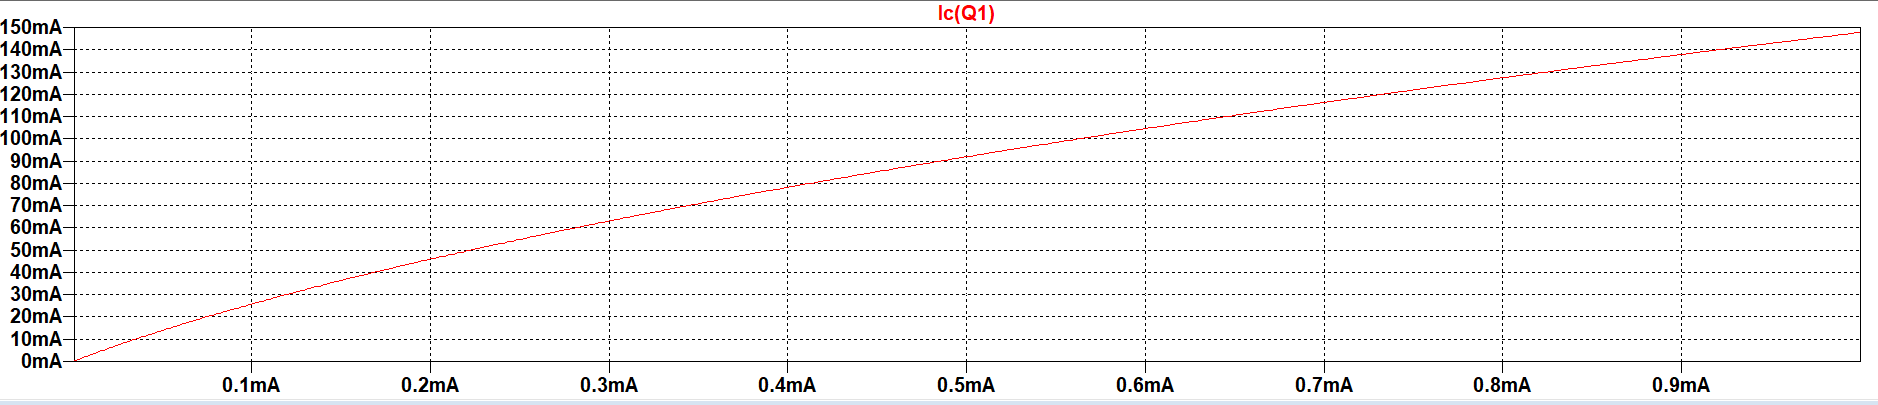
\includegraphics[width=\linewidth]{Bilder/23graph.PNG}
            \caption{Messwerte für den Kollektorstrom \(I_C\)}
        \end{figure}

        Im Graphen ist zu erkennen, dass der Kollektorstrom mit dem Basisstrom zusammen ansteigt. Dies geschieht jedoch nicht linear, sondern hat eine leichte Kurvenform.

    \section{Bestimmung der Stromverstärkung}
        Die Daten für \(I_B\) und \(I_C\) müssen mit LT-Spice aus dem Graphen entnommen werden.\\
        Link!!!!!!!!!!\\
        Durch die Formel
        \begin{equation}
            \beta=\frac{I_C}{I_B}
        \end{equation}
        kann nun die Stromverstärkung ausgerechnet werden. Durch das Logarithmieren von \(I_C\) und \(\beta\) kann die Stromverstärkung als Funktion des Kollektorstroms in einem Diagramm dargestellt werden.

        \begin{figure}[!ht]
            \centering
            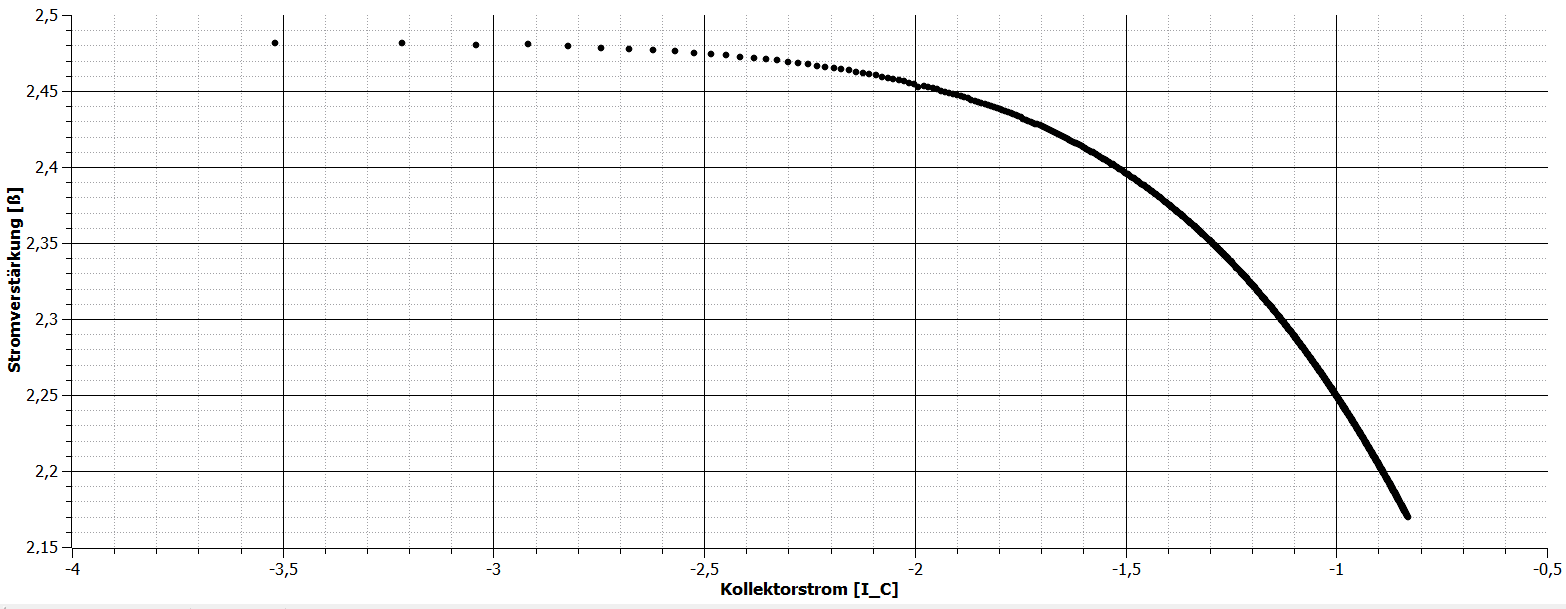
\includegraphics[width=\linewidth]{Bilder/24graph.PNG}
            \caption{Stromverstärkung als Funktion des Kollektorstroms doppellogarithmisch dargestellt}
            \label{fig:241}
        \end{figure}

        Im oben stehenden Link sind die einzelnen Messwerte und Ergebnisse für die Stromverstärkung und die einzelnen logarithmischen Funktionen zu sehen.

        \begin{figure}[!ht]
            \centering
            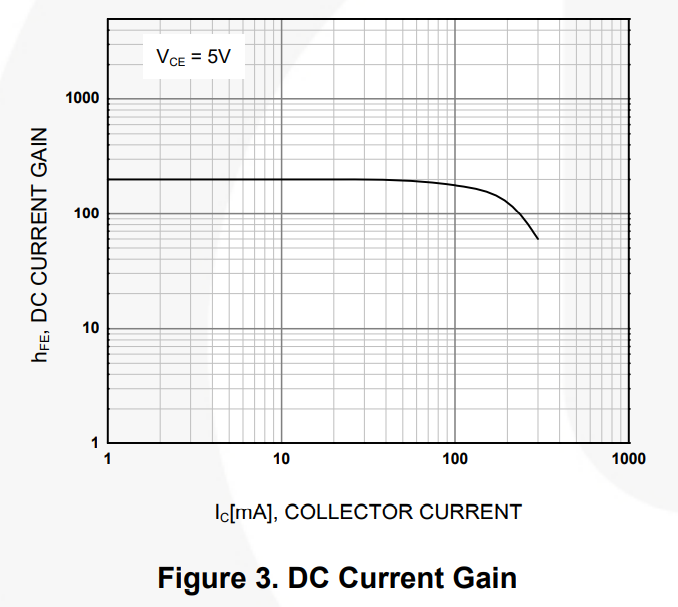
\includegraphics[]{Bilder/24datenblatt.PNG}
            \caption{Graph aus dem Datenblatt des Transistors BC547B \textbf{[B~\ref{fig:242}]}}
            \label{fig:242}
        \end{figure}

        Beim vergleichen der beiden Graphen~\ref{fig:241} und~\ref{fig:242} ist zu erkennen das diese fast gleich verlaufen. Beide laufen anfangs recht linear und ab einem bestimmtenKollektorstrom sinkt die Stromverstärkung rapide ab. Im Graph ~\ref{fig:241} von beiden Achsen der Logarithmus genommen und dann aufgetragen, im Graph ~\ref{fig:242} wurde das ganze im Graphen logarithmisch aufgezeichnet. Das Ergebnis ist das selbe.
        \newpage

    \section{Aufnahme der Ausgangskennlinienschar}
        Bei der Aufnahme der Kennlinienschar wird der gleiche Aufbau wie~\ref{fig:22} verwendet. Jedoch werden nun der Basisstrom I1 \(I_B\) und die Spannungsquelle V1 \(U_{CE}\) als veränderliche Größen verwendet. \(U_{CE}\) wird im Intervall von 0V bis 30V verändert und \(I_B\) im Intervall von 20 \(\mu A\) bis 100 \(\mu A\). Bei \(I_B\) wird schrittweise um 20 \(\mu A\) erhöht.

        \begin{figure}[!ht]
            \centering
            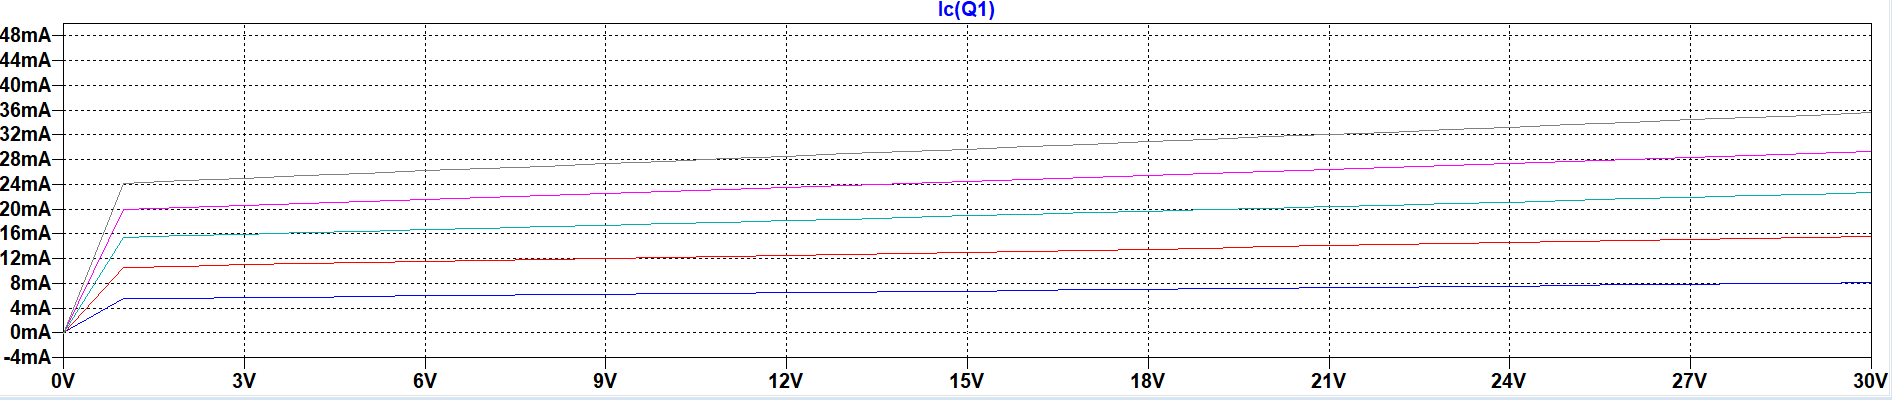
\includegraphics[width=\linewidth]{Bilder/25graph1.PNG}
            \caption{Ausgangskennlinien der verschiedenen Basisstromstärken}
            \label{fig:251}
        \end{figure}

        Aus dem Datenblatt des Transistors BC547B ist folgender Graph zu entnehmen.

        \begin{figure}[!ht]
            \centering
            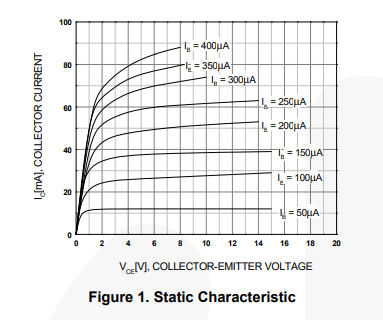
\includegraphics[]{Bilder/25datenblatt.PNG}
            \caption{Graph aus dem Datenblatt von BC547B \textbf{[B~\ref{fig:252}]}}
            \label{fig:252}
        \end{figure}

        Der von LT-Spice ermittelte Graph sieht nur ansatzweise so aus wie der Graph aus dem Datenblatt. Der ermittelte Kollektorstrom (Y-Achse) entspricht nicht den Werten aus dem Datenblatt. Jedoch sind die Intervalle für den Basisstrom im Intervall von $50-100\mu A$ anders gewählt als in unserer Simulation. Deshalb kommen auch die anderen Werte für den Kollektorstrom zustande.\\
        Im folgenden Graph ist noch die Verlustleistungshyperbel für die Schaltung aufgezeigt.

        
        \begin{figure}[!ht]
            \centering
            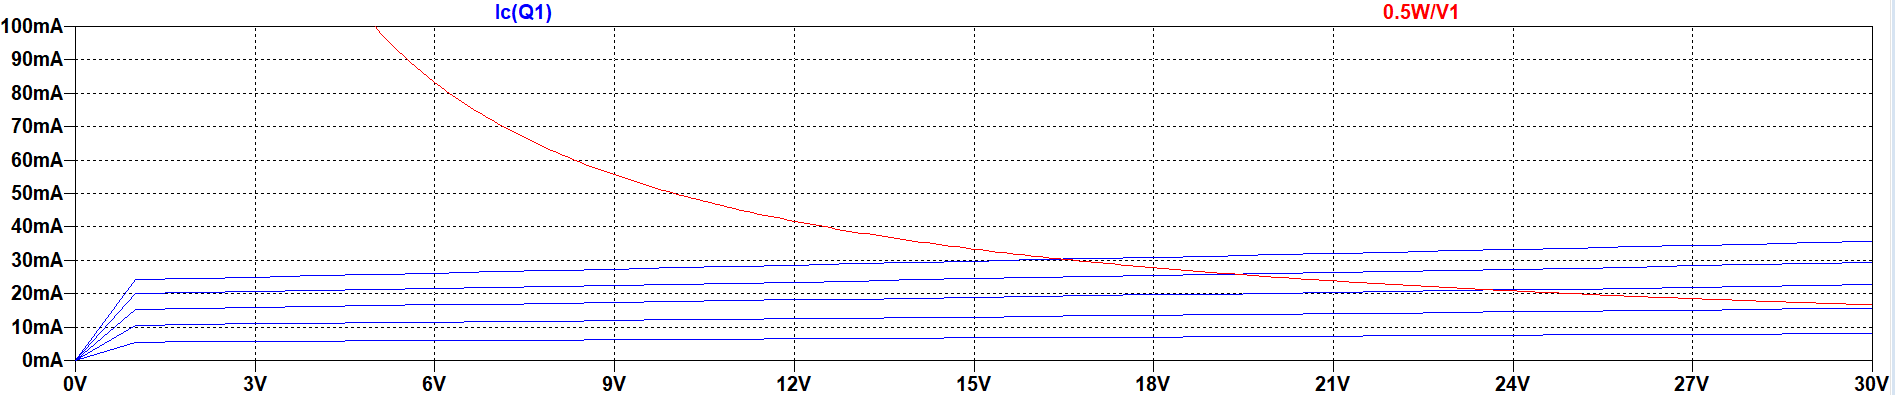
\includegraphics[width=\linewidth]{Bilder/25Verlustl.PNG}
            \caption{Verlustleistungshyperbel}
        \end{figure}

    \section{Bestimmung des differentiellen Ausgangswiderstands}
        Um den differentiellen Ausgangswiderstand \(r_{CE}\) wird die Simulation mit V1 (\(U_{CE}\)) im Intervall von 4V bis 6V und \(I_B\) im Intervall von 50\(\mu A\) bis 350\(\mu A\) in 50\(\mu A\) durchgeführt. Für $I_C$ kommen dabei folgende werte heraus. \\
        Link!!!!!!!!!\\

        Durch die Formel 
        \begin{equation}
            r_{CE}=\frac{\Delta U_{CE}} {\Delta I_C}
        \end{equation}
        lässt sich der Ausgangswiderstand berechnen.

        Da der Strom immer von 4V auf 6V steigt ist $\Delta U_{CE}= 2V$

        Für die den Kollektorstrom $\Delta I_C$ ergeben sich durch das Subtrahieren des Kollektorstroms bei U=4V und U=6V folgende Werte.
        \begin{equation}
            \Delta I_C=I_{Cmax}-I_{Cmin}
        \end{equation}

        \begin{table}[!ht]
        \centering
            \caption{Simulationsergebnisse $\Delta I_C$}
            \begin{tabular}{|c|c|}
                \hline
                \(I_B\) & Wert in A\\ \hline \hline
                50\(\mu A\) & 0.0004223 \\ \hline
                100\(\mu A\) & 0.00078471\\ \hline
                150\(\mu A\) & 0.00110695\\ \hline
                200\(\mu A\) & 0.00139995\\ \hline
                250\(\mu A\) & 0.00167042\\ \hline
                300\(\mu A\) & 0.00192287\\ \hline
                350\(\mu A\) & 0.00216047 \\ \hline
            \end{tabular}
        \end{table}

        Durch das Einsetzen der berechneten Werte in die Formel (1.2) ergibt sich für \(r_{CE}\):
        \begin{table}[!ht]
            \centering
            \caption{Simulationsergebnisse \(\Delta I_C\)}
            \begin{tabular}{|c|c|}
                \hline
                \(I_B\) & Wert von \(r_{CE}\) in \(\Omega\)\\
                \hline \hline
                50\(\mu A\) & 4736 \\ \hline
                100\(\mu A\) & 2549\\ \hline
                150\(\mu A\) & 1807\\ \hline
                200\(\mu A\) & 1429\\ \hline
                250\(\mu A\) & 1197\\ \hline
                300\(\mu A\) & 1040\\ \hline
                350\(\mu A\) & 926\\ \hline
            \end{tabular}
        \end{table}
        \newpage
        Im Folgenden ist der Ausgangswiderstand \(r_{CE}\) in Abhängigkeit von dem Basisstrom \(I_B\) aufgetragen.

        \begin{figure}[!ht]
            \centering
            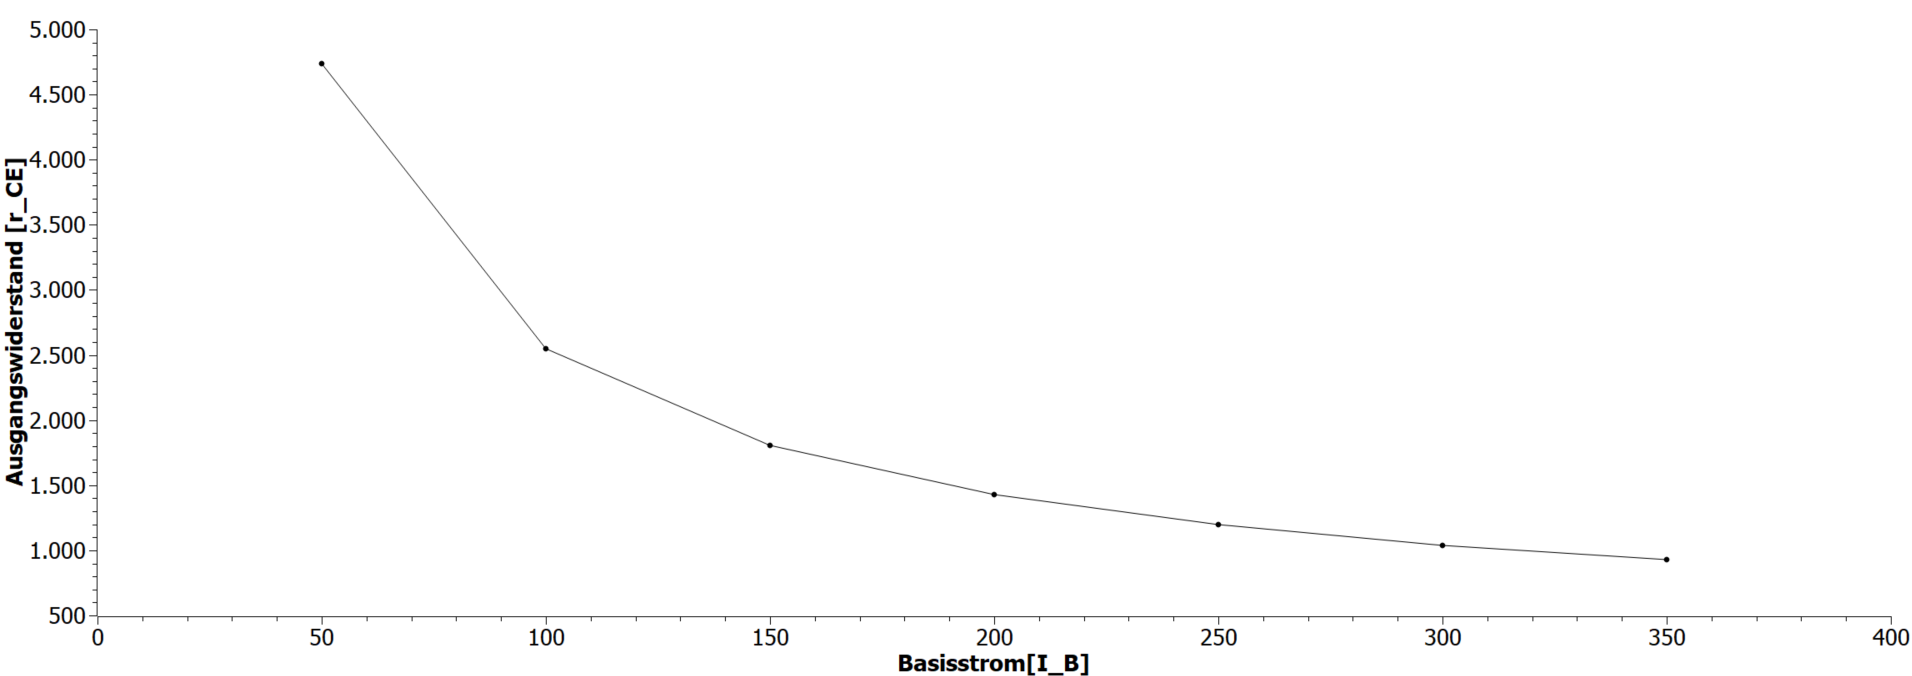
\includegraphics[width=\linewidth]{Bilder/26.PNG}
            \caption{Verhalten des Ausgangswiderstandes zum Basisstrom}
        \end{figure}








